\documentclass{thesis_utf8}

\usepackage{relsize}
\newcommand*{\defeq}{\stackrel{\text{def}}{=}}

\usepackage{enumitem}

\begin{document}
\maketitlepage{Погода Михайло Володимирович}
    {КМ-31М}
    {завідувач кафедри, д-р техн. наук, доцент Чертов~О.\,Р.}
    {професор Тарасенко~В.\,П.}
    {Пошук шаблонів у цифровому сигналі за допомогою поліномів Кунченка}
\pagestyle{plain}
\annotation{Анотація}
Метою цієї магістерської дисертації є розробка та оптимізація програмного комплексу для пошуку шаблонів у цифровому
сигналі.
Комплекс, що розробляється, призначений для виділення ділянок цифрового сигналу, що містять деякий шаблон, можливо у
модифікованому вигляді.

Розглянуто існуючі методи пошуку шаблонів у цифрових сигналах на прикладі нормалізованої кросс"=кореляції та суми
квадратів відстаней, запропонований новий метод і проаналізовані шляхи покращення його роботи.
Розроблений комплекс протестований на низці тестових даних, в тому числі на аудіосигналах з мовленням.

Робота складається з вступу, \total{chapter}  розділів та висновків і налічує \total{page} сторінок.
Містить \total{figurecount} ілюстративних матеріалів, \total{tablecount} таблиць, \total{appendnum} додатки та
посилається на \total{bibitemcount} літературних джерел.

Ключові слова: пошук шаблонів, цифровий сигнал, обробка сигналів, розпізнавання, математичний метод, поліноми
Кунченка.
\clearpage

\annotation{Abstract}
In this paper, the system for template matching in digital signal was developed and optimised.
Program was designed to correctly match subintervals of signal to some template that may be altered in some way.

Also described existing methods for template matching in digital signals such as normalised cross"=correlation and sum
of squared distances, new method was proposed.
Ways for optimisation for new method were observed.
Developed software was tested alongside with existing methods on speech signal.

The work consists of an introduction, \total{chapter} sections, includes conclusions and \total{page} pages.
Contains \total{figurecount} illustrative materials, \total{tablecount} tables, \total{appendnum} appendices and has
\total{bibitemcount} references.

Keywords: template matching, digital signal, signal processing, recognition, mathematical algorithm, Kunchenko
polynomials.

% vim: spelllang=uk,en spell

\tableofcontents
\shortings{}

\todo[inline]{Fill list of shortings (25 left)}
% vim: spelllang=uk,en spell

\intro{}
Інтелектуальна обробка інформації вже дуже давно зарекомендувала себе в сучасному світі.
Людство генерує незчисленні обсяги інформації щосекунди.
Багато згенерованої інформації (поки що) не зберігається, а з того, що зберігається, багато ніяк не аналізується.

Але з поширенням інформаційних технологій та з розповсюдженням пристроїв, що можуть ефективно обробляти великі обсяги
інформації, знаходиться все більше сфер, де можливо отримати користь з раніш не оброблюваного інформаційного потоку.

Наприклад, аналізуючи зміни погодних умов упродовж дня, метеорологи мають змогу прогнозувати погоду наперед;
аналізуючи різні показники життєдіяльності людини, лікарі знаходять прояви хвороб ще до перших її симптомів.

Задачі пошуку окремих наперед визначених властивостей чи образів у деякому масиві даних набули великого поширення в
галузях, пов’язаних з обробкою цифрової інформації.

Співставлення з еталоном (template matching) широко застосовується в аналізі як одновимірних, так і двовимірних
сигналів~\cite{book4}.

Зазвичай, постановка такої задачі включає в себе дані для аналізу, деякий шаблон для пошуку та, можливо, область, на
якій потрібно здійснювати такий пошук.  При цьому потрібно як правильно обрати представлення вхідних даних, так і
визначити критерії, за якими відбуватиметься зіставлення шаблону з сигналом~\cite{book10}.

Існує розмаїття підходів та метрик, які можна використовувати для вирішення цієї задачі.

У даній роботі для цього пропонується використовувати поліноми Кунченка.

% vim: spelllang=uk,en spell

\chapter{Постановка задачі}
% TODO: Описати постановку задачі
% vim: spelllang=uk,en spell

\chapter{Огляд існуючих методів}

Оскільки задача пошуку шаблонів у сигналах була поставлена дуже давно, існує багато методів пошуку шаблону в сигналі.
Ці методи різняться за областю застосування, швидкодією, чутливістю до різних перетворень шаблону.

В цьому розділі будуть розглянуті основні існуючі методи:
\begin{itemize}
    \item Взаємокореляція;
    \item Нормалізована взаємокореляція;
    \item Сума квадратів відстаней;
    \item Нормалізована сума квадратів відстаней.
\end{itemize}

Буде проведений порівняльний аналіз методів й обґрунтована доцільність дослідження обраного методу.

\section{Опис предметної області}
    В цьому підрозділі будуть описані загальні терміни, що будуть необхідні при описі методів.

    Ми будемо використовувати в якості сигналу довільну функцію
    \[f:\:\mathbb{X} \rightarrow \mathbb{Y},\] де множина вихідних значень $\mathbb{Y} \in \mathbb{R}$, а множина
    вхідних значень $\mathbb{X} \in \mathbb{R}$ для одновимірного сигналу, $\mathbb{X} \in \mathbb{R}^2$ для двовимірного сигналу, тощо.

    Під цифровим сигналом будемо розуміти функцію $f^*$, що задана співвідношеннями:
    \begin{eqnarray*}
        f^*(x_0) &=& y_0\\
        f^*(x_1) &=& y_1\\
        \dots\\
        f^*(x_n) &=& y_n
    \end{eqnarray*}
    Такі функції ще називають таблично"=заданими, оскільки вони можуть бути записаними у вигляді таблиці.

    Наприклад, для цифрового звукового сигналу, множина $\{x_i\}$ представляє собою моменти часу, в яких визначені
    амплітуда звукового сигналу $\{y_i\}$.
    % TODO s/"=/"=/g
    Для цифрового чорно"=білого зображення з розмірами $600 \times 400$ пікселів, область визначення цифрового сигналу
    буде множина пар
    \[\{ (a, b) \}, a \in \{1,2,\dots,599,600\}, b \in \{1,2,\dots,399,400\}\]
    Областю значень сигналу може бути, наприклад, $\{0,1,2,\dots,254,255\}$, де значення $0$ має чорний піксель, а
    $255$ --- білий.

    З кожної функції $f(x)$ можна утворити безліч таблично"=заданих функцій, вибравши з області визначення цієї
    функції скінченну підмножину $\{x_i\}$ й співставивши цієї підмножині відповідні значення функції $\{f(x_i)\}$.
    Такий процес ще називається дискретизацією сигналу.
    Якщо в якості вхідного сигналу виступає сигнал, що залежить від часу (наприклад, аудіо"=сигнал), за умови, що $|
    x_i - x_{i-1}| = \delta$, то частотою дискретизації називають співвідношення $\frac{1\,c}{\delta}$.

    \subsection{Метод ковзаючого вікна}
    \label{ss:sliding-window}
        Оскільки задача пошуку шаблону в цифровому сигналі ставиться як пошук наперед визначеного шаблону (або його
        трансформацій) в дискретному сигналі, що має (набагато) більшу довжину, то в методах пошуку шаблонів
        використовується метод ковзаючого вікна.

        Цей метод полягає в розбитті вхідного сигналу на \invcommas{вікна} --- неперервні ділянки, кожна з яких має
        одну й ту саму довжину.
        Як правило, довжина вікна дорівнює довжині шаблону, а самі вікна накладаються одне на одного.
        Для кожного вікна шукається міра подібності вмісту вікна до шаблону.

        Таким чином будується функція $e(x)$, яка характеризує подібність вікна, що задається параметром $x$ до
        шаблону.
        З цієї функції можна оцінювати найвірогідніші позиції шаблону.

        Така оцінка, як правило, робиться шукаючи локальні екстремуми, які вище/нище якогось порогу $e_{0}$.

\section{Опис існуючих методів}
    \subsection{Взаємокореляція}
        Взаємокореляція (cross-correlation) являє собою міру подібності двох функцій (сигналів), одна з яких
        зсувається відносно іншої.

        Для дискретного сигналу взаємокореляція має вигляд:
        \begin{equation}
            CC(f,g)[ n ] \equiv (f \star g)[ n ] \defeq \frac{1}{k}\sum\limits_{m=1}^{k} f^*[m] g[ m + n ]
        \end{equation}

        Для використання цього методу необхідно взяти в якості сигналу $f$ вхідний сигнал, $g$ --- шаблон, що
        шукається; в якості $k$ необхідно взяти довжину (кількість значень) шаблону $g$.

        Ідея полягає в тому, що сума добутків значень шаблону на вхідний сигнал буде тим більше, чим більше вхідний
        сигнал схожий на шаблон на обраному проміжку.

        Значним недоліком цього методу є залежність від амплітуди сигналу: якщо сигнал має на деякому проміжку
        амплітуду, значно більшу за середню амплітуду сигналу та шаблону, то значення взаємокореляції між сигналом та
        шаблоном на цьому проміжку буде значно більше, ніж значення взаємокореляції між шаблоном та шаблоном
        (автокореляція).

        Саме тому більш практичним вважається використання нормалізованої взаємокореляції.
    \subsection{Нормалізована взаємокореляція}
        Нормалізована взаємокореляція шукається як взаємокореляція між сигналами, що нормалізовані.
        Як правило, під нормалізацією розуміється віднімання від сигналу середнього значення на проміжку й ділення на
        середньо"=квадратичне відхілення на цьому проміжку.

        Для дискретного сигналу нормалізована взаємокореляція має вигляд:
        \begin{eqnarray}
            NCC(f,g)[ n ] &\defeq& \frac{1}{k} \sum\limits_{m=1}^{k} \tilde{f_n}^*[m] \tilde{g}[ m + n ],\\
            \tilde{f_n}[m] &\defeq& \frac{f[m] - \bar{f_n}}{\sigma_{f_n}},\\
            \tidle{g}[m]   &\defeq& \frac{g[m] - \bar{g}}{\sigma_g}
        \end{eqnarray}
        де $\sigma_{f_n}$ --- середньо"=квадратичне відхілення вікна вхідного сигналу $f$, $\sigma_g$ ---
        середньо"=квадратичне відхилення шаблону $g$, $\bar{f_n}$ --- середнє значення вхідного сигналу на проміжку
        вікна, а $\bar{g}$ --- середнє значення шаблону.

        Цей метод дозволяє знаходити шаблон, навіть якщо вхідний сигнал має значні \invcommas{спалахи} амплітуди.
        Також нормалізація шаблону дозволяє знаходити в сигналі шаблон із зміненої амплітудою.

        Завдяки тому, що значення цієї метрики лежать в межах від ${-1}$ до $1$, задача пошуку порогу $e_0$ значно
        спрощується.

    \subsection{Сума квадратів відстаней}
        Метод полягає в пошуку квадрату відстані між $k$"=вимірного вектору шаблону та обраного вікна сигналу.

        Для дискретного сигналу це буде наступна залежність:
        \begin{equation}
            \text{SSD}\left(f, g\right)[ n ] \defeq \frac{1}{k}\sum\limits_{m=1}^k {\left(f[m] - g[m]\right)}^2
        \end{equation}

        Отримана функціональна залежність характеризує відстань кожного вікна вхідного сигналу до шаблону.
        Таким чином, чим менше ця відстань --- тим більше сигнал у обраному вікні схожий до шаблону.

        На відміну від методу взаємокореляцій, на ефективність методу пошуку суму квадратів відстаней не впливає
        значення амплітуди сигналу.
    \subsection{Нормалізована сума квадратів відстаней}
        Аналогічно до нормалізованої взаємокореляції можна визначити нормалізовану суму квадратів відстаней:
        \begin{equation}
            \text{NSSD}\left(f, g\right)[ n ] \defeq \frac{1}{k}\sum\limits_{m=1}^k {\left(\tilde{f}[m] - \tilde{g}[m]\right)}^2
        \end{equation}

\section{Порівняльний аналіз методів}
\label{s:existing-compare}
    В таблиці~\ref{tab:existing} підсумовані основні характеристики розглянутих методів.
    Слід зазначити, що підрахування взаємокореляції можна значно прискорити завдяки (швидкому) перетворенню Фур’є
    (FFT).

    \stepcounter{tablecount}
    \begin{table}{|p{0.1\textwidth}|p{0.2\textwidth}|p{0.3\textwidth}|p{0.29\textwidth}|}
        {Порівняння існуючих методів}{tab:existing}
        {\hline
            &
Складність обчислень &
Стійкість до зміни амплітуди шаблону &
Стійкість до артефактів вхідного сигналу\\
        \hline}

        CC   & $O(k n)$   & $-$ & $-$\\
        NCC  & $O(2 k n)$ & $+$ & $+$\\
        SSD  & $O(k n)$   & $-$ & $+$\\
        NSSD & $O(2 k n)$ & $+$ & $+$\\
    \end{table}

    Як можна побачити, найпоширеніші методи, що застосовуються для сигналів загального виду, є дуже чутливими до
    зміни шаблону: тільки метод нормалізованої взаємокореляції дозволяє коректно знаходити шаблон із лінійно"=зміненою
    амплітудою.
    \todo[inline]{Вставити посилання}
    Експерименти показали, що ці методи не знаходять шаблон в сигналі, якщо амплітуда шаблону змінювалася не сталим
    чином.

\section{Висновки}
    \todo[inline]{Обґрунтування обраного методу}

% vim: spelllang=uk,en spell filetype=tex

\chapter{Опис обраного методу}
\section{Лінійній простір Кунченко}
\todo[inline]{Лінійній простір Кунченко}
\subsection{Розклад довільної функції у просторі Кунченко}
\todo[inline]{Розклад довільної функції у просторі Кунченко}

\section{Застосування розкладення для пошуку шаблону в сигналі}
\todo[inline]{Застосування розкладення для пошуку шаблону в сигналі}
\subsection{Опис алгоритму пошуку шаблонів}
\todo[inline]{Опис алгоритму пошуку шаблонів}
\subsection{Методи прискорення пошуку шаблонів}
\todo[inline]{Методи прискорення пошуку шаблонів}

% vim: spelllang=uk,en spell

\chapter{Проектування програмних засобів}
\section{Вибір програмного середовища}
\todo[inline]{Вибір програмного середовища}
\section{Проектування архитектури програмної реалізації}
\todo[inline]{Проектування архитектури програмної реалізації}
\section{Алгоритм роботи програми}
\todo[inline]{Алгоритм роботи програми}
% vim: spelllang=uk,en spell


\chapter{Математичне моделювання та статистичний експеримент}
\label{chap:testing}

\section{Пошук у синтетичному сигналі}
    В цьому підрозділі розглянемо пошук шаблону в сигналі, що був згенерований як певна композиція неперервних
    функцій.

    \subsection{Пошук шаблону без модифікацій}
        Для початку порівняємо методи пошуку шаблонів використовуючи сигнал із шаблоном, котрий був доданий без
        будь"=яких видозмінень (окрім адитивного шуму/трансформації).

        В рамках експерименту на проміжку ${[0; 10]}$ із частотою дискретизації 10~КГц будувався сигнал, що складався
        з 8--16 гаусіан нормального розподілу $\dfrac{1}{\sigma\sqrt{2\pi}}
        e^{\frac{{\left(x-\mu\right)}^2}{2\sigma^2}}$
        (кількість гаусіан і їх параметри обиралися випадковим чином).
        До цього сигналу (бази) у випадкову позицію додавався шаблон виду $\sin{\alpha x^2}$.
        Приклад такого сигналу наведений на рисунку~\ref{fig:a-1}.
        На рисунку~\ref{fig:a-3} наведені відповідні ефектограми нормалізованої взаємокореляції, нормалізованої суми
        квадратів відстаней та методу на основі поліномів Кунченко.

        \todo[inline]{Вписати дані після застосування пірамідального пошуку}

        \stepcounter{tablecount}
        \begin{table}
            {|p{0.2\textwidth}|C{0.2\textwidth}|C{0.27\textwidth}|p{0.15\textwidth}|}
            {Результати пошуку шаблону без модифікації}
            {tab:a-1}
            {\hline
                         & Час, с & Абсолютна похибка & Екстремум\\
                \hline}
            Kunchenko & 108,01 & -0,04 & 0,06\\
            NCC       & 5,55   & -0,04 & 0,25\\
            NSSD      & 5,51   & -0,04 & 1.50\\
        \end{table}


        \stepcounter{figurecount}
        \begin{figure}[h]
            \centering
            \subfloat[Без шуму]{%
                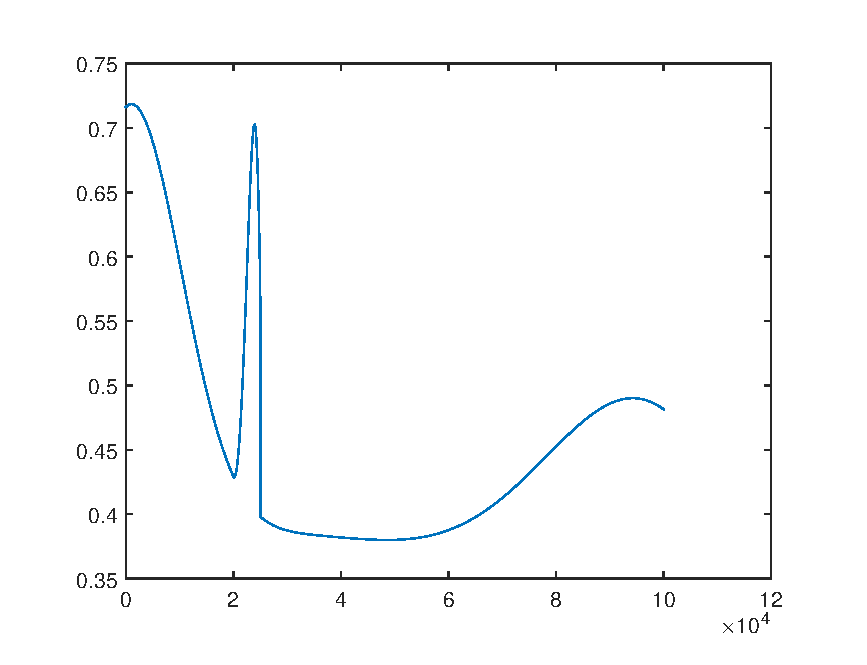
\includegraphics[width=0.8\textwidth]{a_1.eps}
            }

            \subfloat[Із шумом]{%
                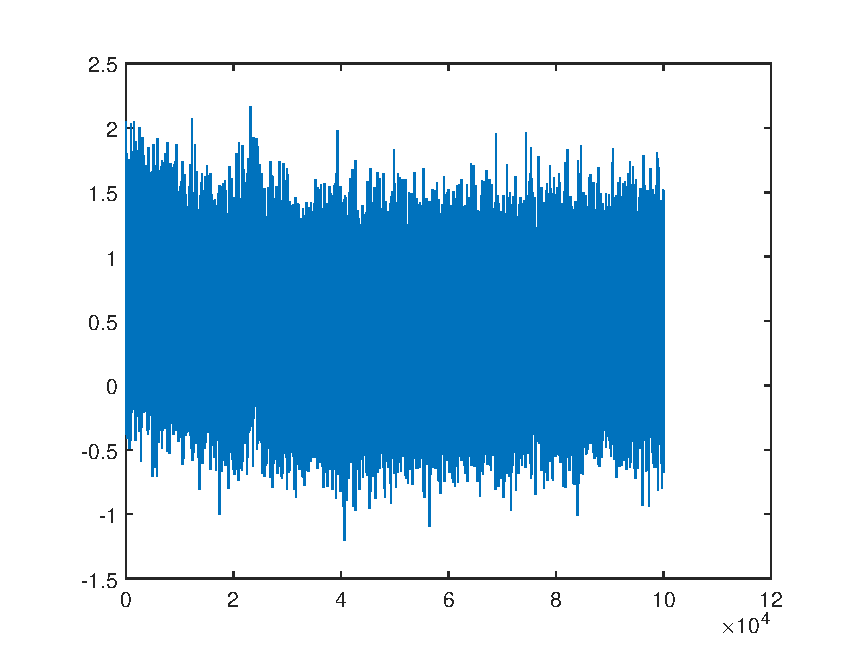
\includegraphics[width=0.8\textwidth]{a_2.eps}
            }
            \caption{Приклад сигналу із шаблоном без модифікації}\label{fig:a-1}
        \end{figure}

        \stepcounter{figurecount}
        \begin{figure}[!h]
            \centering
            \subfloat[Kunchenko]{%
                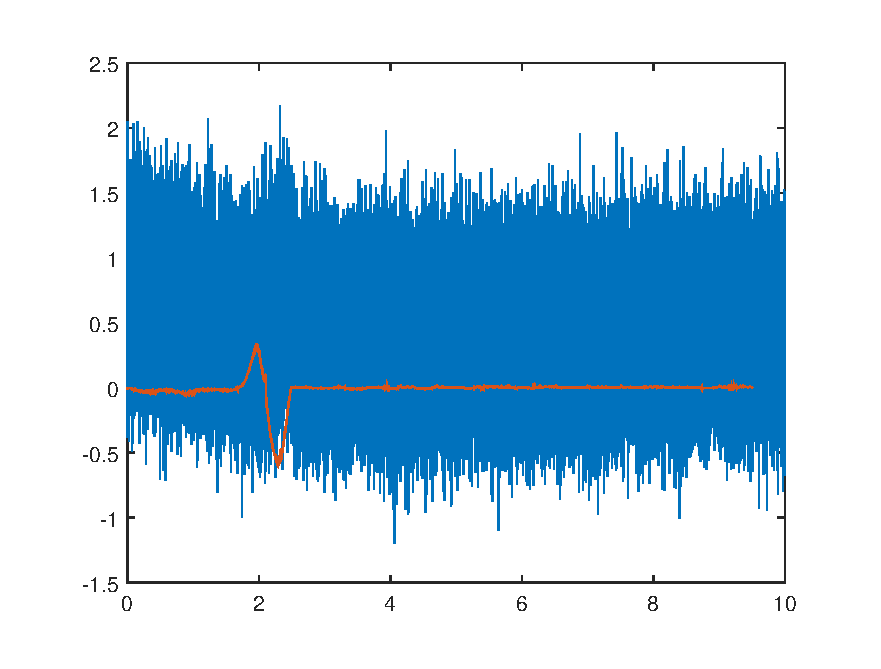
\includegraphics[height=0.28\textheight]{a_3.eps}
            }

            \subfloat[NCC]{%
                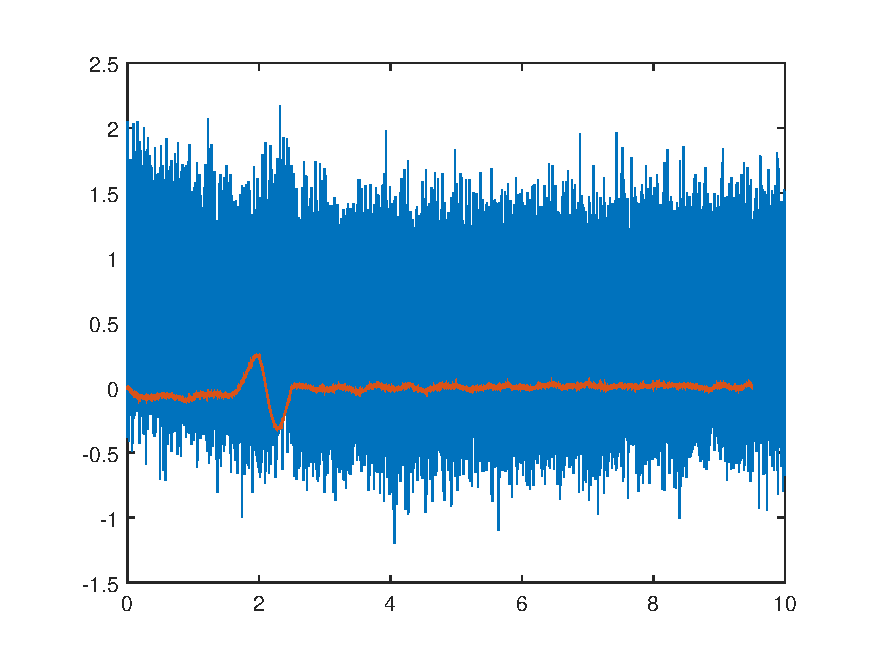
\includegraphics[height=0.28\textheight]{a_4.eps}
            }

            \subfloat[NSSD]{%
                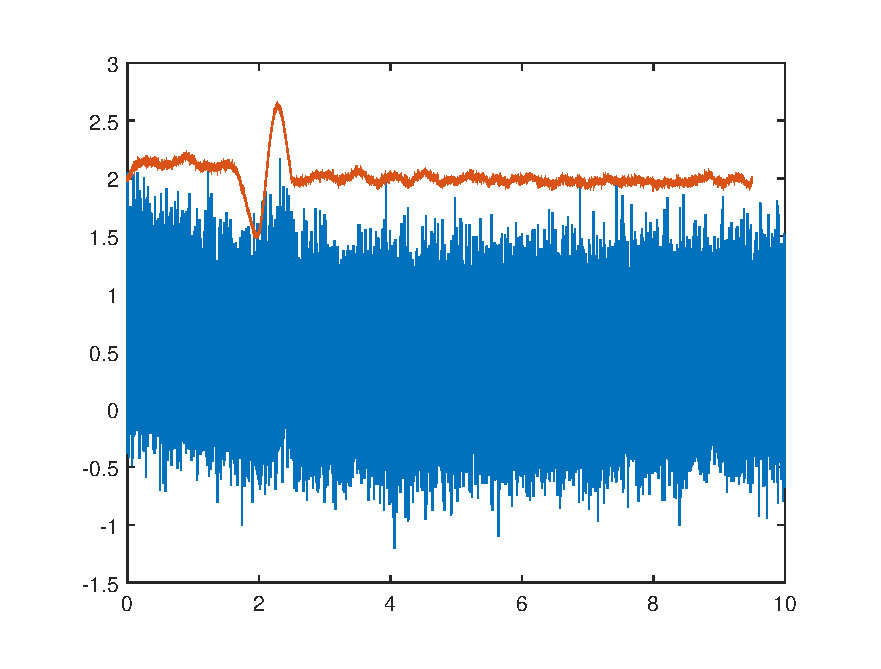
\includegraphics[height=0.28\textheight]{a_5.eps}
            }
            \caption{Пошук шаблона без модифікацій в синтетичному сигналі}\label{fig:a-3}
        \end{figure}
        У таблиці~\ref{tab:a-1} приведені дані статистичного експерименту.

    \subsection{Пошук шаблону з модифікацій}
    \todo[inline]{Привести дані статистичного експерименту №2}
\section{Пошук шаблону у мовленнєвому сигналі}
Протестуємо метод Кунченко для пошуку шаблона (аудіозапис слова) в сигналі.
\todo[inline]{Описати експеримет й його результати}
\stepcounter{figurecount}
\begin{figure}[!h]
    \centering
    \subfloat[Сигнал]{%
        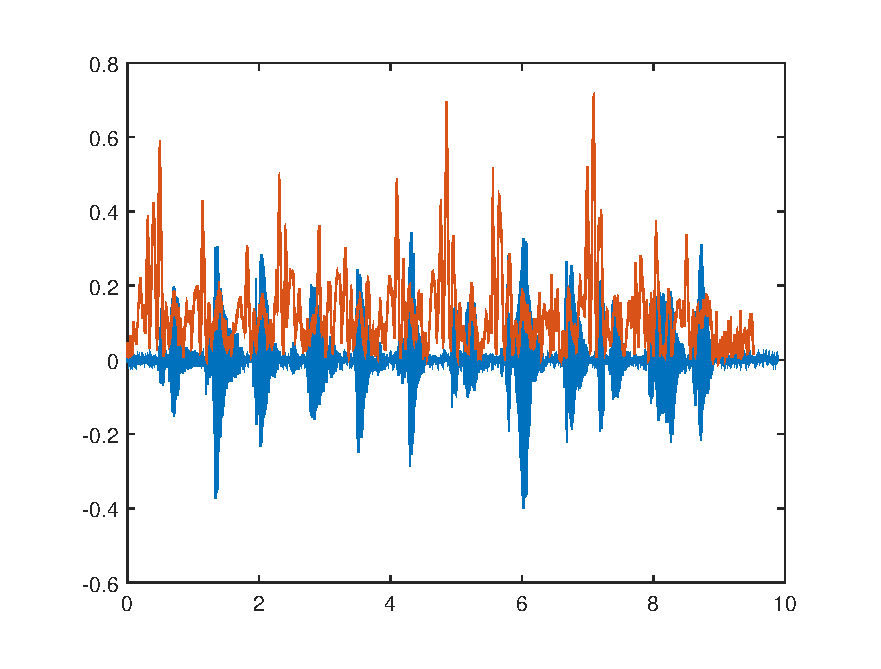
\includegraphics[width=0.8\textwidth]{audio.eps}
    }

    \subfloat[Зразок]{%
        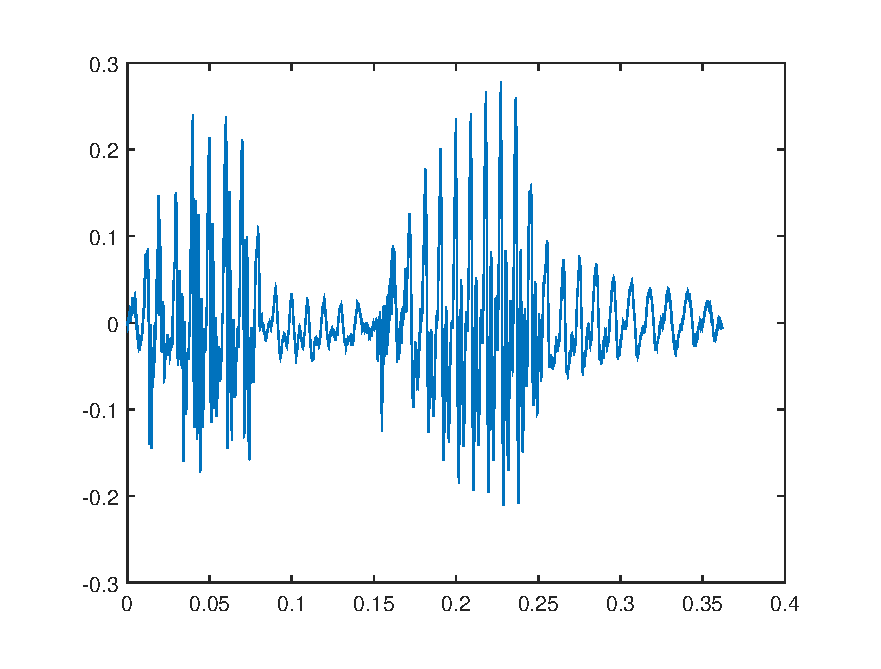
\includegraphics[width=0.8\textwidth]{audio_template.eps}
    }
    \caption{Запис мовлення й шаблон для пошуку}\label{fig:audio}
\end{figure}

\stepcounter{figurecount}
\begin{figure}[!h]
    \centering
    \subfloat[Kunchenko]{%
        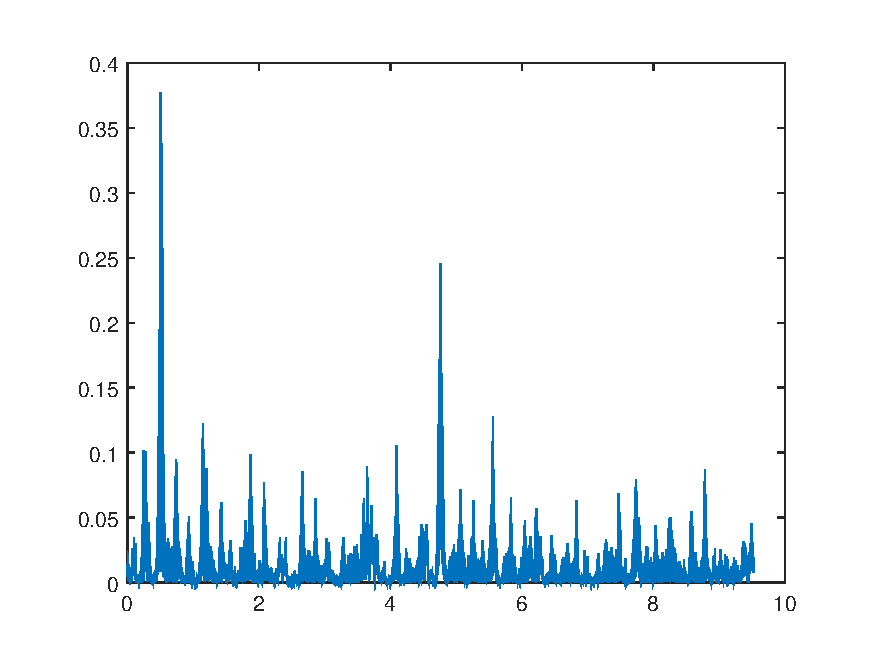
\includegraphics[height=0.28\textheight]{matched_plain_kun.eps}
    }

    \subfloat[NCC]{%
        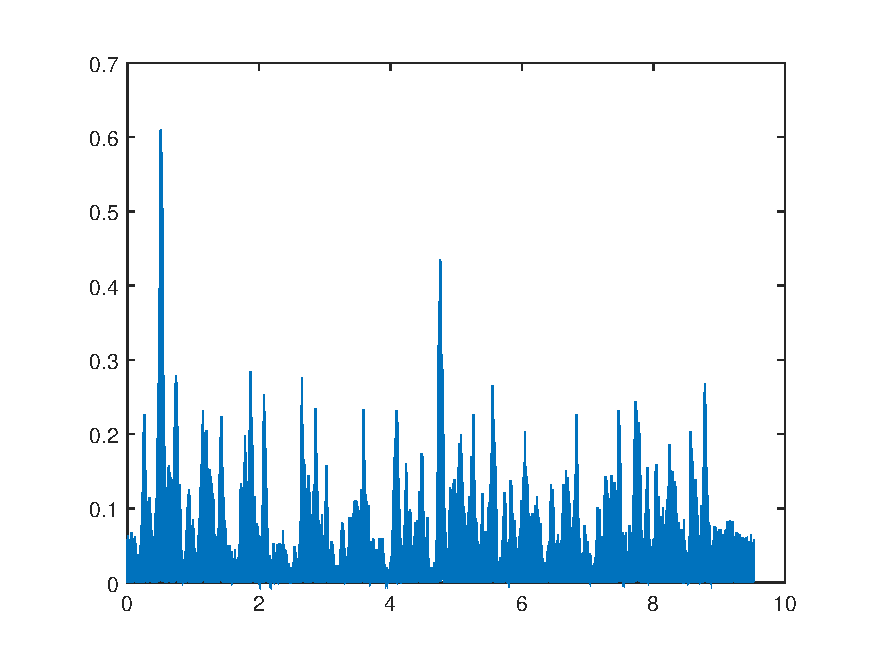
\includegraphics[height=0.28\textheight]{matched_plain_ncc.eps}
    }

    \subfloat[NSSD]{%
        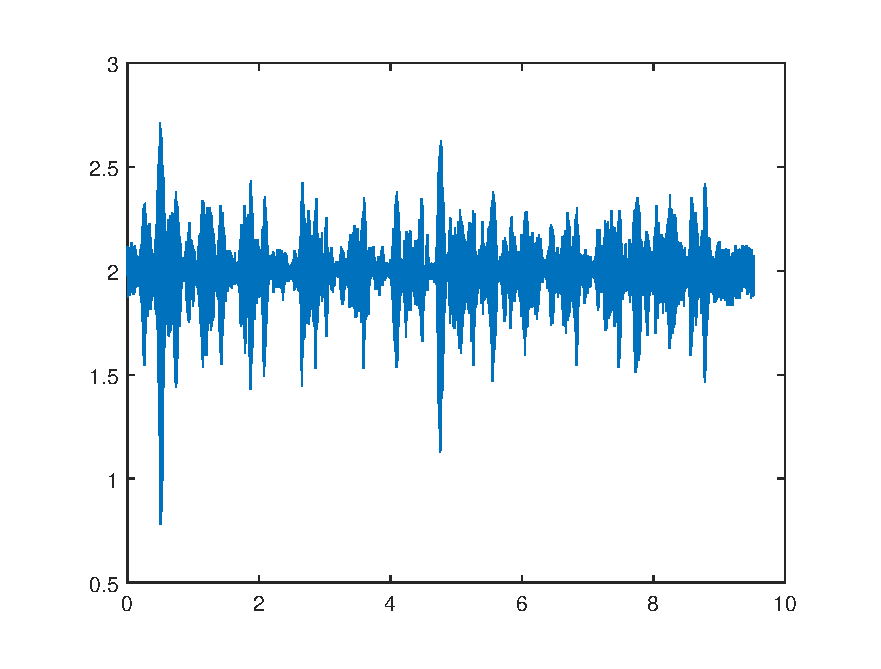
\includegraphics[height=0.28\textheight]{matched_plain_ssd.eps}
    }
    \caption{Знайдений шаблон в сигналі}\label{fig:matched-plain-audio}
\end{figure}

\stepcounter{figurecount}
\begin{figure}[!h]
    \centering
    \subfloat[Сигнал]{%
        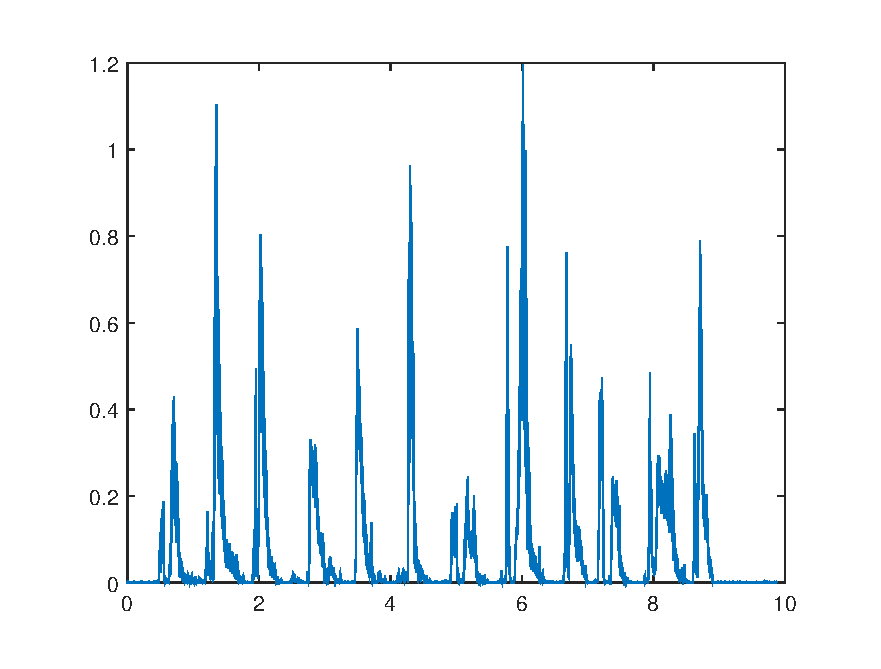
\includegraphics[width=0.8\textwidth]{audio_energy.eps}
    }

    \subfloat[Зразок]{%
        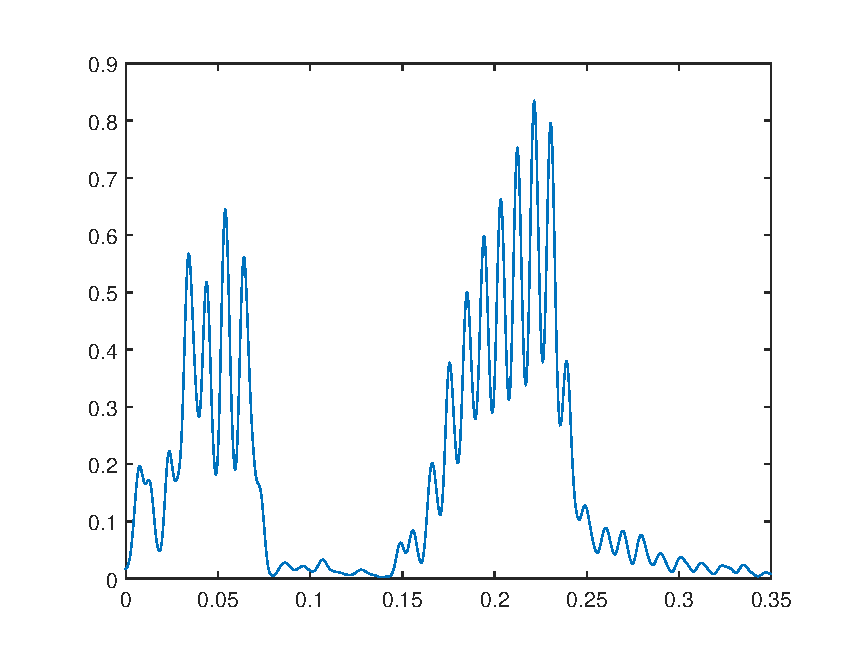
\includegraphics[width=0.8\textwidth]{audio_template_energy.eps}
    }
    \caption{Короткочасна енергія запису мовлення й шаблону для пошуку}\label{fig:audio-energy}
\end{figure}

\stepcounter{figurecount}
\begin{figure}[!h]
    \centering
    \subfloat[Kunchenko]{%
        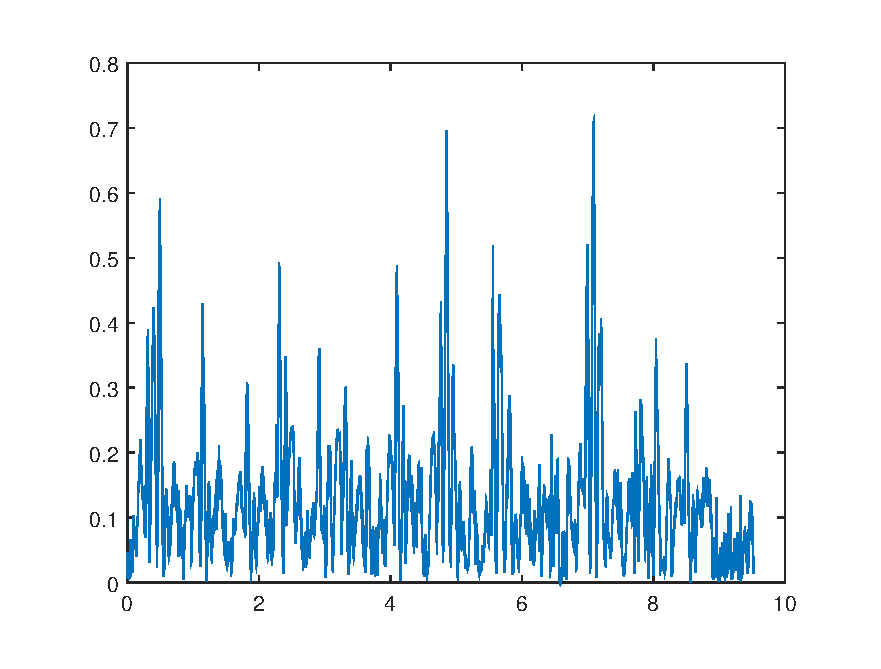
\includegraphics[height=0.28\textheight]{matched_energy_kun.eps}
    }

    \subfloat[NCC]{%
        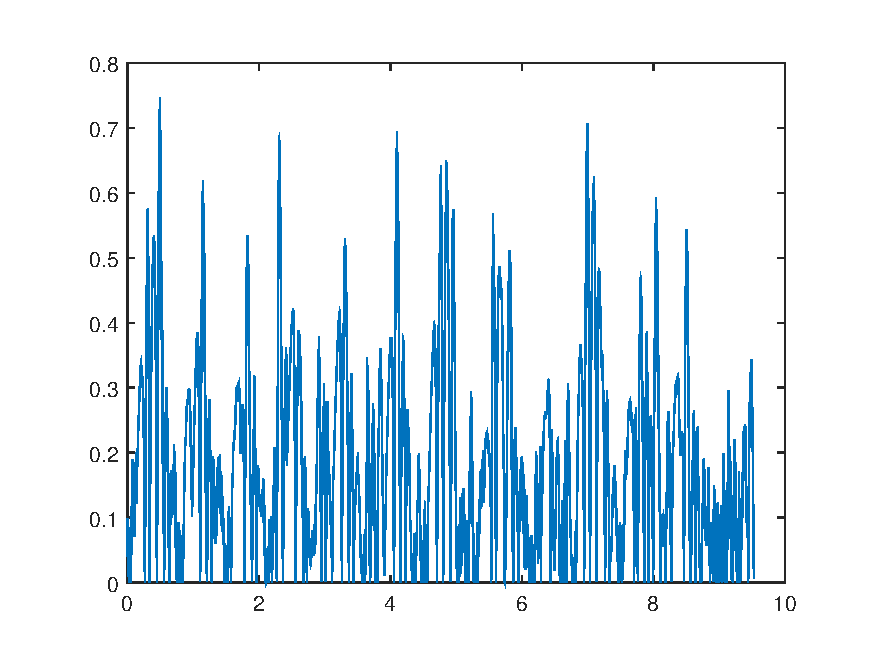
\includegraphics[height=0.28\textheight]{matched_energy_ncc.eps}
    }

    \subfloat[NSSD]{%
        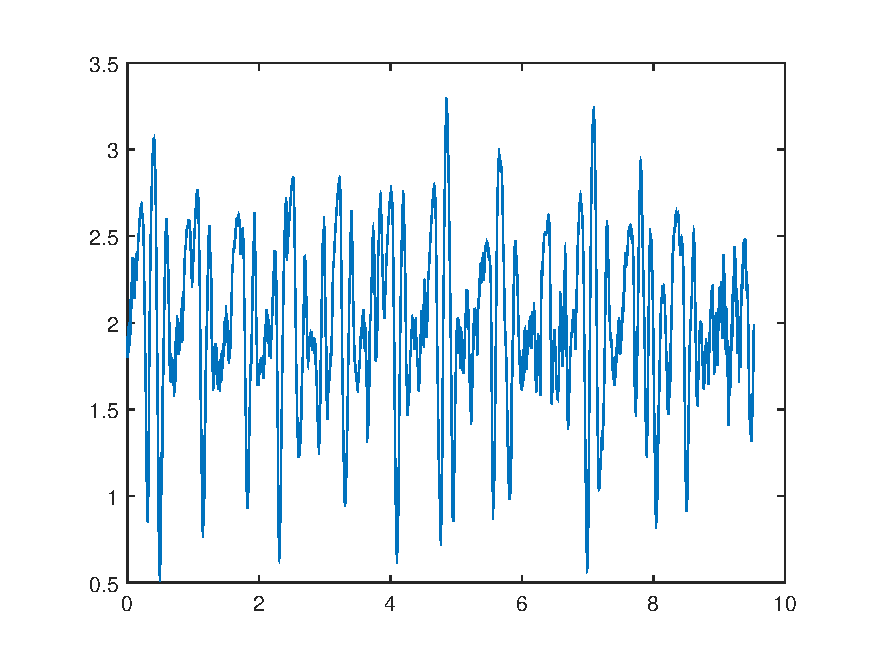
\includegraphics[height=0.28\textheight]{matched_energy_ssd.eps}
    }
    \caption{Знайдений шаблон в енергії сигналу}\label{fig:matched-energy-audio}
\end{figure}
% ncc-energy = 2.5
% ssd-energy = 2.4
% kun-energy = 86
% ncc = 2.52
% ssd = 2.85
% kun = 87



% vim: spelllang=uk,en spell filetype=tex


\lstset{breakatwhitespace=false
       ,breaklines=true
       ,commentstyle=\rm
       ,escapeinside={\%*}{*)}
       ,frame=none
       ,language=Matlab
       ,stringstyle=\rm
       ,title=\lstname
       }

\conclusion{}
В магістерській дисертації розглядалася задача пошуку шаблонів у цифрових сигналах.
В ході дослідження було проаналізовані існуючі методу для пошуку шаблонів і порівняні їх обмеження.

Під час огляду предметної області були розглянуті такі поняття, як цифровий сигнал, кросс"=кореляція, сума квадратів
відстаней, метод ковзного вікна та віконні функції.
Розглянуті віконні функції було використано при тестуванні в методі ковзного вікна.

Був запропонований метод пошуку шаблонів, що базується на розкладанні функції в базисі лінійного функціонального
простору Кунченка.
Відмінною особливістю цього методу є можливість пошуку шаблонів, що були значно змінені в сигналі.

Також були запропоновані шляхи покращення роботи методу на основі поліномів Кунченка.
Пірамідальний пошук дозволяє значно прискорити роботу методу, оскільки він дозволяє відфільтрувати значну частину
сигналу як таку, що не містить шаблону, за досить короткий проміжок часу.
Використання методів оптимізації також дозволяють значно прискорити роботу алгоритму.

Був розроблений та оптимізований програмний комплекс в математичному середовищі MathWorks MATLAB 2014b.

Під час статистичного експерименту було порівняно ефективність роботи обраного методу з існуючими методами як на
штучно"=згенерованому сигналі, так і для аудіозапису мовлення.
Як результат цього тестування можна зазначити, що обраний метод дозволяє отримати аналогічну ступінь розпізнавання на
штучно"=згенерованих сигналах і значно вищу якість на аудіозаписах мовлення.

Для пошуку шаблону в аудіозаписі з мовленням було використано визначення коротко"=часової енергії й віконних функцій.
Було проаналізовано поведінку алгоритму в залежності від обраних параметрів методу.

Для подальшого розвитку слід зазначити можливість дослідження методів інтелектуального вибору параметрів алгоритму в
залежності від характеристик сигналу, апаратне прискорення для більш швидкої роботи алгоритму та апробація методу на
даних з іншої предметної області.

\begin{thebibliography}
    \stepcounter{bibitemcount}
    \bibitem{book1}% посилання на книжку
    Vanderbrug, G.J. and Rosenfeld, A. (1977) Two-stage Template Matching. IEEE Transactions on Computers, C-26, 102--103.

    \stepcounter{bibitemcount}
    \bibitem{book2}% посилання на книжку
    Rosenfeld, A. and Vanderbrug, G.J. (1977) Coarse-Fine Template Matching. IEEE Transactions on Systems, Man and Cybernetics, 7, 104-107.

    \stepcounter{bibitemcount}
    \bibitem{book3}% посилання на книжку
    Ken Turkowski and Steve Gabriel (1990). \invcommas{Filters for Common Resampling Tasks}. In Andrew S. Glassner. Graphics
    Gems I. Academic Press. pp. 147–165. ISBN 978-0-12-286165-9.
\end{thebibliography}

\append{Лістінг реалізації алгоритму пошуку шаблонів}
\lstinputlisting[language=Matlab]{OneDimentionalIterator.m}
\lstinputlisting[language=Matlab]{approximate.m}
\lstinputlisting[language=Matlab]{match.m}
\lstinputlisting[language=Matlab]{calculateOneDimentionalCorrelant.m}
\lstinputlisting[language=Matlab]{ncc.m}
\lstinputlisting[language=Matlab]{ssd.m}
\lstinputlisting[language=Matlab]{energy_sf.m}
\append{Ілюстративні матеріали}
\end{document}
% vim: spelllang=uk,en spell
